%!TEX root =  gettingStartedFAuST-version2_0.tex
\chapter{Introduction}\label{sec:intro}

\paragraph{What is the \FAuST\ toolbox ?} FA$\mu$ST is a C++ toolbox, useful to decompose or approximate any given dense matrix into a product of sparse matrices, in order to reduce its computational complexity (both for storage and manipulation). 
As an example, Figure \ref{fig:presentation} shows a dens matrix \textbf{A} and sparse matrices $\mathbf{S_j}$ such that $\mathbf{A}=\prod_{j=1}^J\mathbf{S_j}$.

\begin{figure}[H] %%[!htbp]
\centering
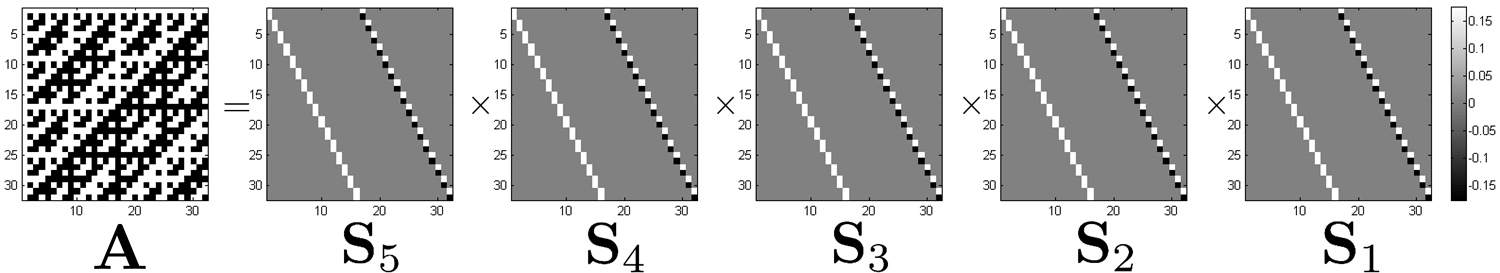
\includegraphics[scale=0.5]{images/hadamard32_bw.pdf}
\caption{Brief presentation of FA$\mu$ST}
\label{fig:presentation}
\end{figure}

\paragraph{Why shall I use \FAuST\ ?} FA$\mu$ST can be used to speed up iterative algorithms commonly used for solving high dimensional linear inverse problems. The algorithms implemented in the toolbox are described in details by Le Magoarou \cite{LeMagoarou2016}. For more information on the FA$\mu$ST project, please visit the website of the project: \url{http://faust.gforge.inria.fr}.


%\paragraph{Brief description:} 
%$A=\prod_{j=1}^J S_j$.

%Valid Installation: Platforms, Compiler and IDE
\paragraph{Is my platform and compiler currently supported ?} 
\FAuST\ has been tested in various configurations, and is currently delivered with a Matlab wrapper. Figure \ref{fig:recapInstall} summarizes the configurations on which \FAuST\ has been tested. 

\paragraph{How should I use this document ?}
If your platform and configuration is currently supported according to Figure \ref{fig:recapInstall}, please refer to the corresponding Install Chapter. By default we suggest the installation using the GCC or Clang compiler directly from a command terminal since it requires fewer externals components. 
\begin{itemize}
\item for installation on UNIX (including Linux and Mac OS X) platform refer to Chapter \ref{sec:InstallUnix};
\item for installation on Windows refer to Chapter \ref{sec:WinInstall}. 
\end{itemize}
Chapter \ref{sec:firstUse} shows quickly how to use this library and gives an example of application. Finally, a "work in progress" part is given Chapter \ref{sec:WorkingProgress} to give an overview of the roadmap for \FAuST. 

\begin{figure}[H] %%[!htbp]
\centering
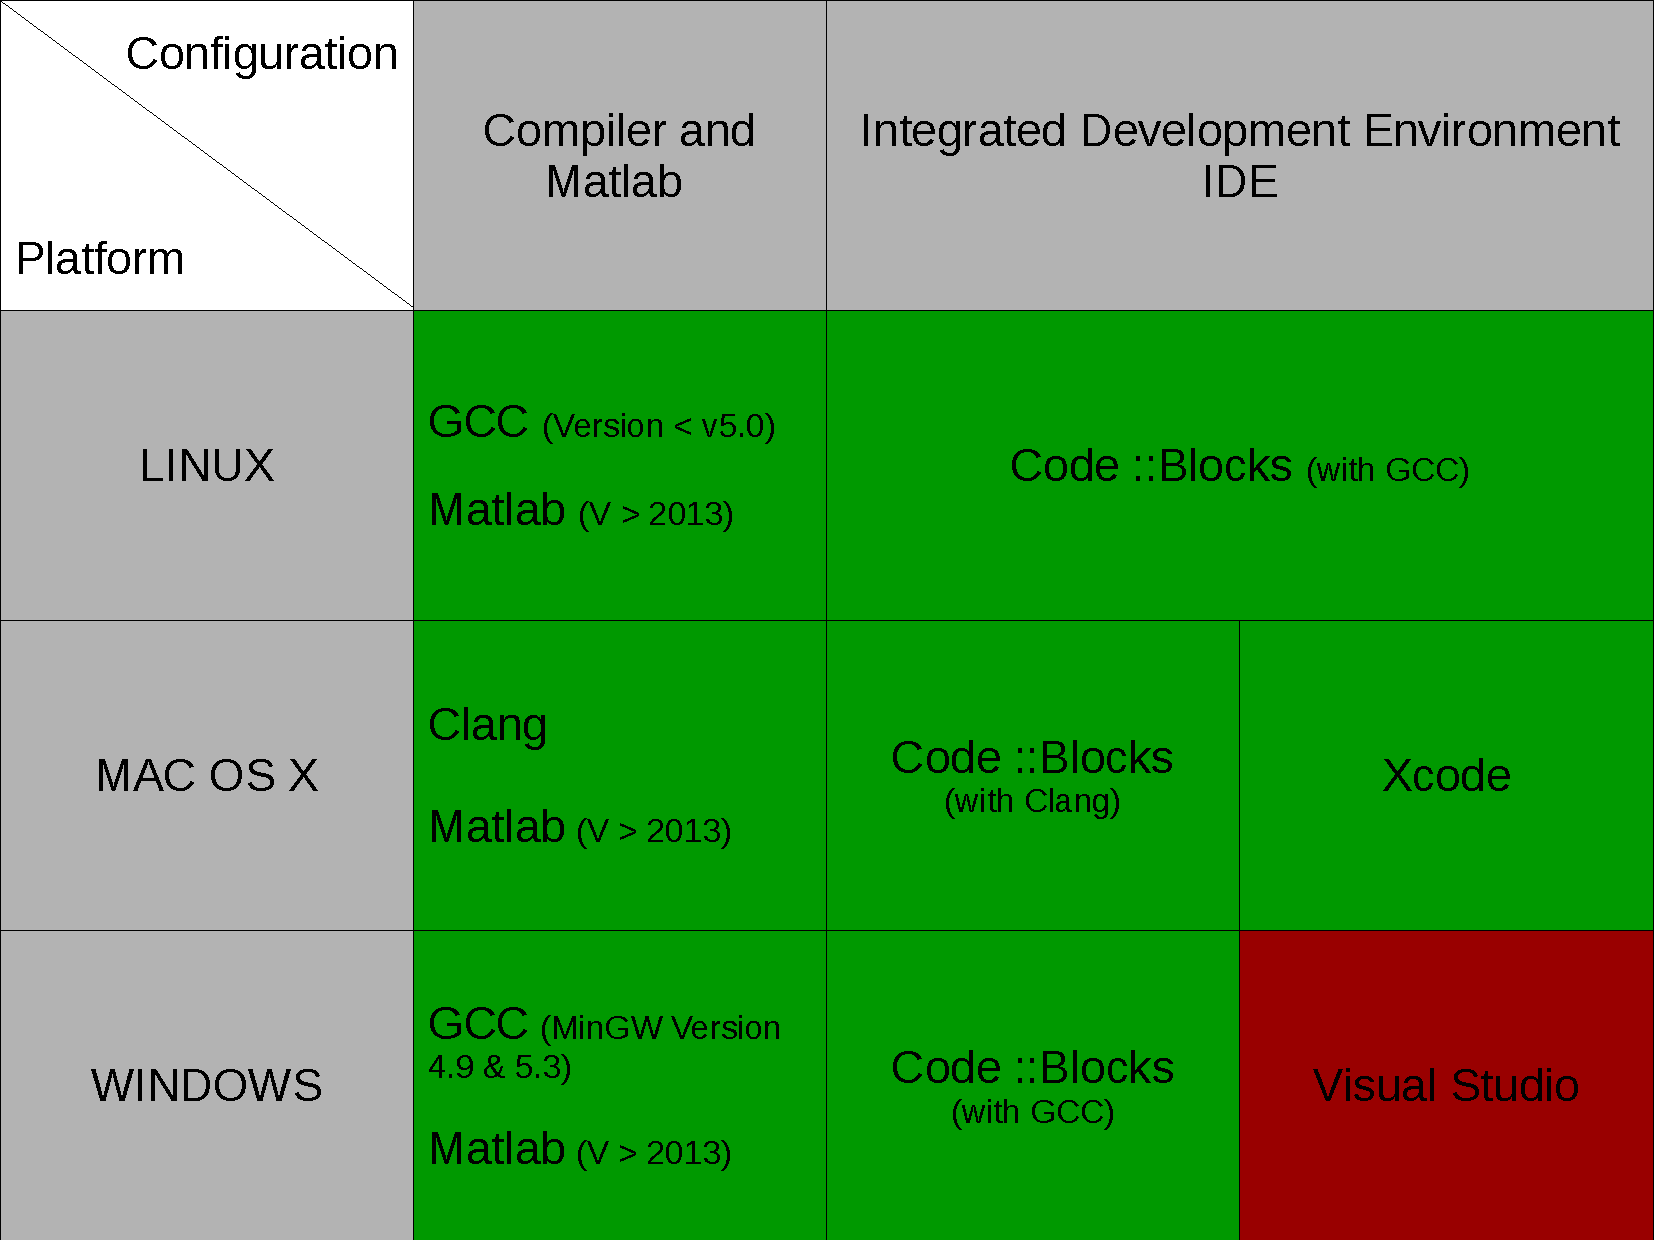
\includegraphics[scale=0.4]{images/recapInstall.pdf}
\caption{Tested configurations: Platforms and IDE}
\label{fig:recapInstall}
\end{figure}

\paragraph{How is the code of \FAuST structured ?}
A brief outline of the code structure and status is given on Figure~\ref{fig:faustStructure}. The main C++ library called \textrm{libfaust} includes two components:
\begin{itemize}
\item the "FA$\mu$ST matrix multiplication" provides efficient linear operators to efficiently manipulate your data, relying on efficient low-level routines from external libraries where needed; 
\item the "Factorization algorithms" is used to generate a FA$\mu$ST core from a dense matrix. 
\end{itemize}
Various wrappers are planned to call \textrm{libfaust}. In the current version of \FAuST\ (Version 2.0), only the Matlab wrapper is implemented. Command-line, Python and A||GO wrapper are planned in the next version of FA$\mu$ST (see Section \ref{sec:WorkingProgress}).   


\begin{figure}[H] %%[!htbp]
\centering
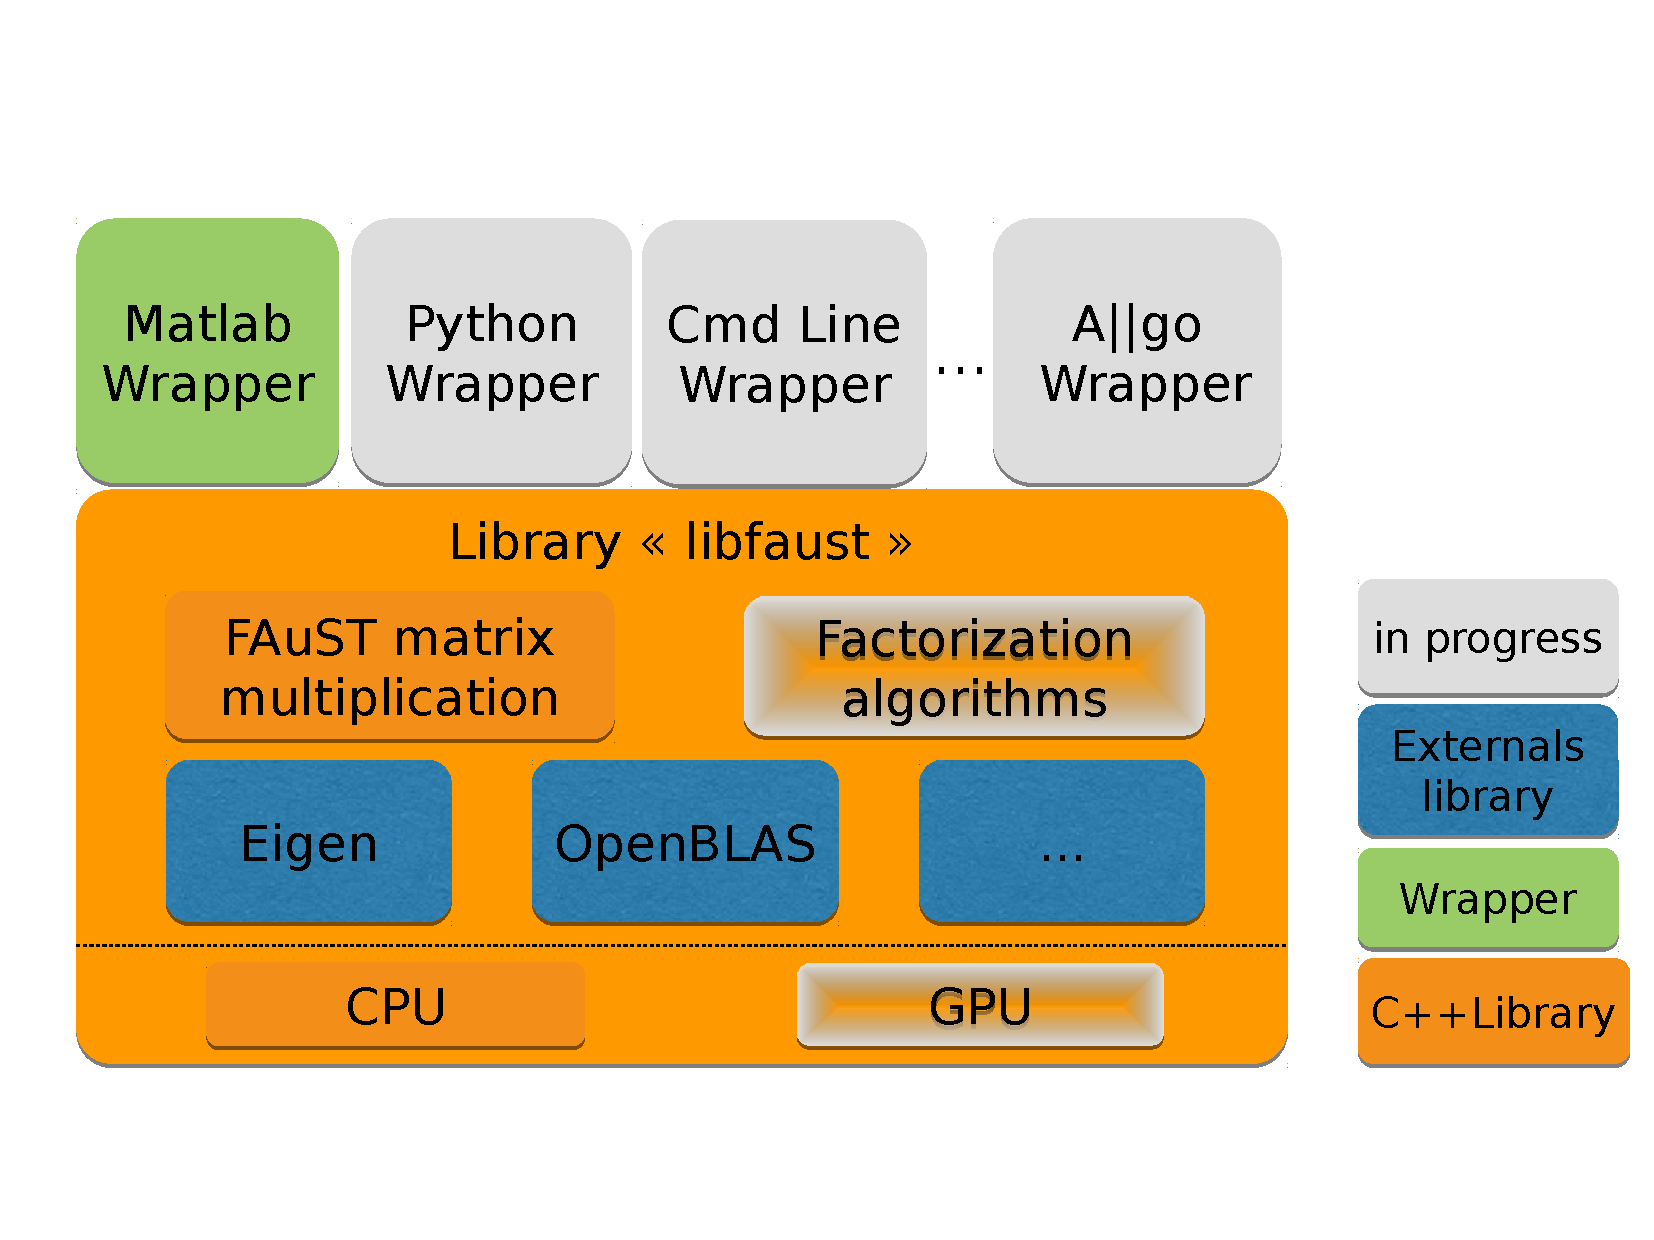
\includegraphics[scale=0.45,trim = 0cm 3cm 0cm 3cm, clip]{images/FaustStructure.pdf}
\caption{Brief structure of FA$\mu$ST version 2.0.0}
\label{fig:faustStructure}
\end{figure}

\paragraph{Known issues :}
\begin{enumerate}
\item The installation on Windows using Visual Studio IDE has been tested with success in certain configurations, however \textbf{compilation problems have been encountered depending on the version of Windows and Visual Studio}. Unfortunately we cannot offer technical support but you may nevertheless report problems and/or suggestions on the mailing list \url{http://lists.gforge.inria.fr/pipermail/faust-install/}. 
 
\item Compiling mex files with the \textbf{mex compiler} of Matlab requires a compatible third-party compiler. \textbf{Warning: With  Matlab Release2016a, the mex compiler seems to only support up to GCC 4.7 (see \url{http://fr.mathworks.com/support/compilers/R2016a/index.html?sec=glnxa64} for more detail)}.

\item The "Factorization algorithms" module represented on Figure \ref{fig:faustStructure} is still work in progress (see Section \ref{sec:WorkingProgress}). A GPU implementation is also on its way, as well as more wrappers.

\end{enumerate}

\paragraph{How do I pronounce \FAuST\ ?} We suggest to pronounce the library name as ``FAUST'', but you may also pronounce it ``FAMUST'' ;-)


\paragraph{License :}Copyright (2016) Luc Le Magoarou, Remi Gribonval INRIA Rennes, FRANCE \\
The FA$\mu$ST Toolbox is distributed under the terms of the GNU Affero General Public License. This program is free software: you can redistribute it and/or modify it under the terms of the GNU Affero General Public License as published by the Free Software Foundation. This program is distributed in the hope that it will be useful, but WITHOUT ANY WARRANTY; without even the implied warranty of MERCHANTABILITY or FITNESS FOR A PARTICULAR PURPOSE.  See the GNU Affero General Public License for more details. You should have received a copy of the GNU Affero General Public License along with this program.  If not, see \url{http://www.gnu.org/licenses/}.
